\documentclass[11pt,a4paper]{article}

% -------------------- Packages --------------------
\usepackage[utf8]{inputenc}
\usepackage[T1]{fontenc}
\usepackage{lmodern}
\usepackage[margin=2.5cm]{geometry}
\usepackage{setspace}
\usepackage{graphicx}
\usepackage{caption}
\usepackage{subcaption}
\usepackage{amsmath,amssymb}
\usepackage{hyperref}
\usepackage{enumitem}
\usepackage{blindtext}
\usepackage{ragged2e}

\setstretch{1.15} 
\setlength{\parskip}{0.5em}
\setlength{\parindent}{0pt}
\geometry{left=1.4cm, top=.8cm, right=1.4cm, bottom=1.8cm, footskip=.5cm}

\renewcommand\thesection{\Roman{section}.}
\renewcommand\thesubsection{\arabic{subsection}.}

\begin{document}

\begin{center}
    {\LARGE \textbf{Research Experiences}}\\[0.8em]
    {\large Junhee Cho}\\[0.5em]
    \normalsize
    Email: \href{mailto:junheecho@postech.ac.kr}{junheecho@postech.ac.kr}
\end{center}

\section{Construction of cryogenic ion trap system for quantum computing}
\hspace{0.5 cm}
\textbf{Affiliation:} Quantum Computing and Quantum Networks (QCQN) laboratory, POSTECH \hfill

\hspace{0.5 cm}
\textbf{Supervisor:} Prof.~Moonjoo Lee

\begin{center}
    \subsection{Design and fabrication of multi-layer ion trap chip}
\end{center}

\begin{figure}[!h]
    \centering
    \includegraphics[width=6 in]{figures/figure1.pdf}
    \caption{
    (\textbf{a})
    Cross-section view of multi-layer trap and Maxwell simulation result on radial plane
    and
    (\textbf{b})
    Fabricated multi-layer ion trap
    }
    \label{fig:figure1}
\end{figure}

\begin{itemize}[leftmargin=2.0em]
    \item 
\end{itemize}

\begin{center}
    \subsection{Construction of cryogenic ion trap system}
\end{center}

\begin{figure}[h]
    \centering
    \includegraphics[width=6 in]{figures/figure2.pdf}
    \caption{
    (\textbf{a})
    Cross-section view of multi-layer trap and Maxwell simulation result on radial plane
    and
    (\textbf{b})
    Fabricated multi-layer ion trap
    }
    \label{fig:figure2}
\end{figure}

\begin{itemize}[leftmargin=2.0em]
    \item 
    \item 
    \item 
\end{itemize}

\begin{center}
    \subsection{Investigation of light-induced charging effect on the trap electrodes}
\end{center}

\begin{figure}[h]
    \centering
    \includegraphics[width=3 in]{figures/figure3.pdf}
    \caption{
    (\textbf{a})
    Cross-section view of multi-layer trap and Maxwell simulation result on radial plane
    and
    (\textbf{b})
    Fabricated multi-layer ion trap
    }
    \label{fig:figure3}
\end{figure}

\begin{itemize}[leftmargin=2.0em]
    \item 
    \item 
    \item 
\end{itemize}

\begin{center}
    \subsection{CNN-based detection program for trapped ions}
\end{center}

\begin{figure}[h]
    \centering
    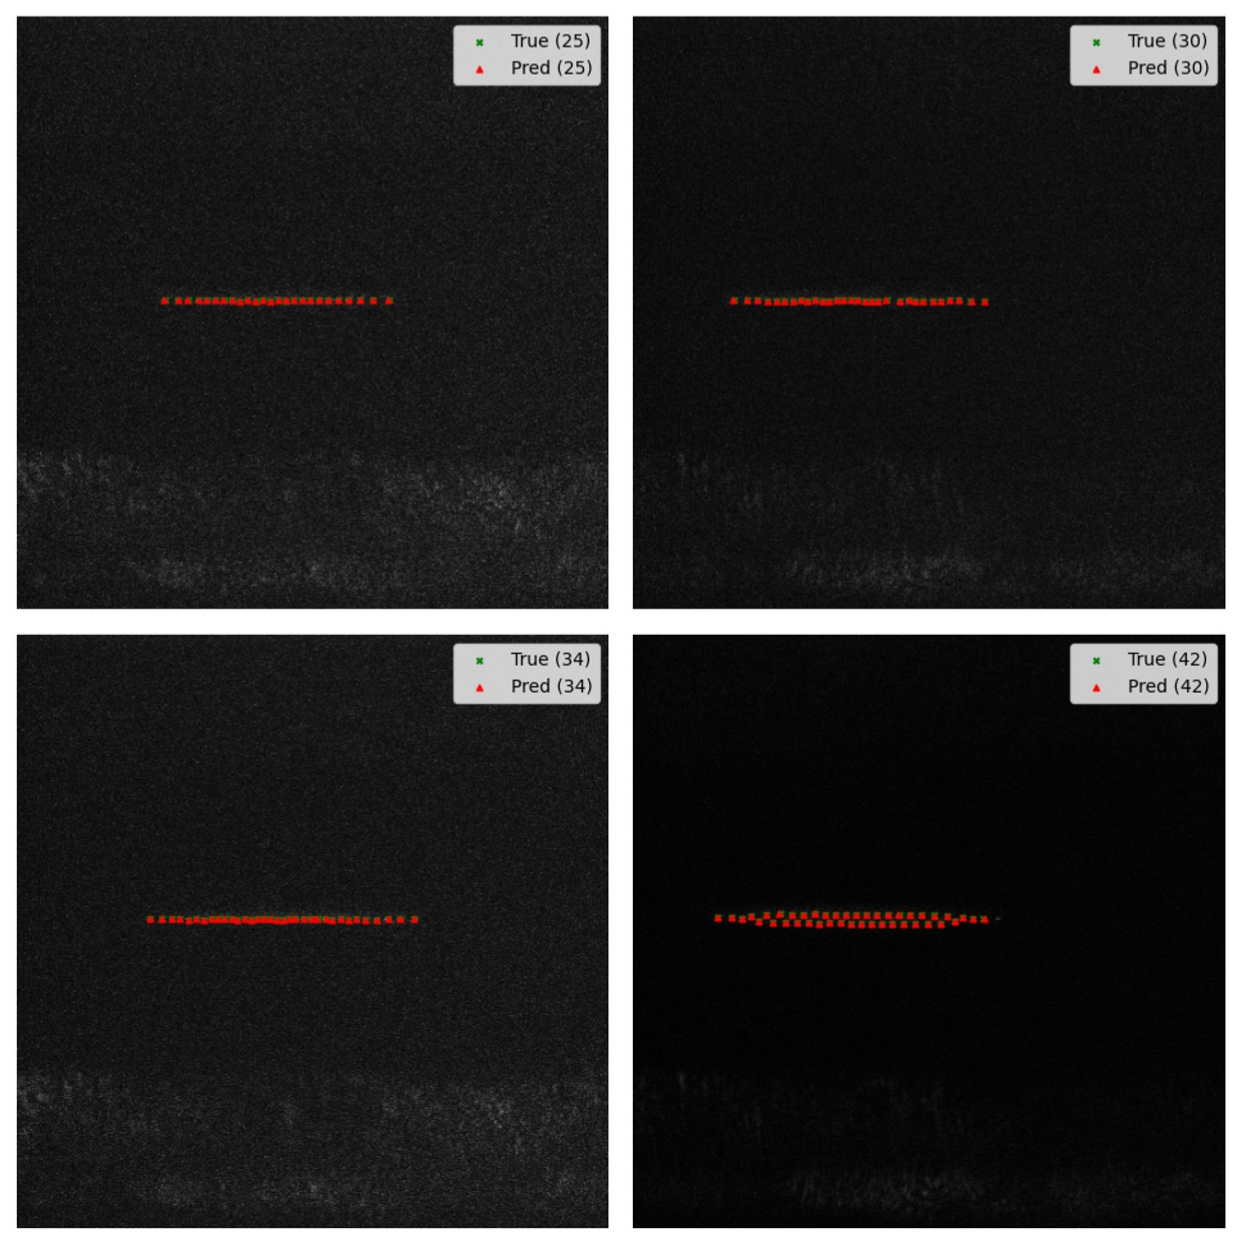
\includegraphics[width=3 in]{figures/figure4.pdf}
    \caption{
    (\textbf{a})
    Cross-section view of multi-layer trap and Maxwell simulation result on radial plane
    and
    (\textbf{b})
    Fabricated multi-layer ion trap
    }
    \label{fig:figure4}
\end{figure}

\begin{itemize}[leftmargin=2.0em]
    \item 
    \item 
    \item 
\end{itemize}

\section{Normally-off GaN MOS-HFET}
\hspace{0.5 cm}
\textbf{Affiliation:} Advanced Semiconductor Technology Lab.(ASTL) laboratory, Hongik University \hfill

\hspace{0.5 cm}
\textbf{Supervisor:} Prof.~Ho-young Cha

\begin{center}
    \subsection{Modeling normally-on GaN/AlGaN HEMT}
\end{center}

\begin{figure}[h]
    \centering
    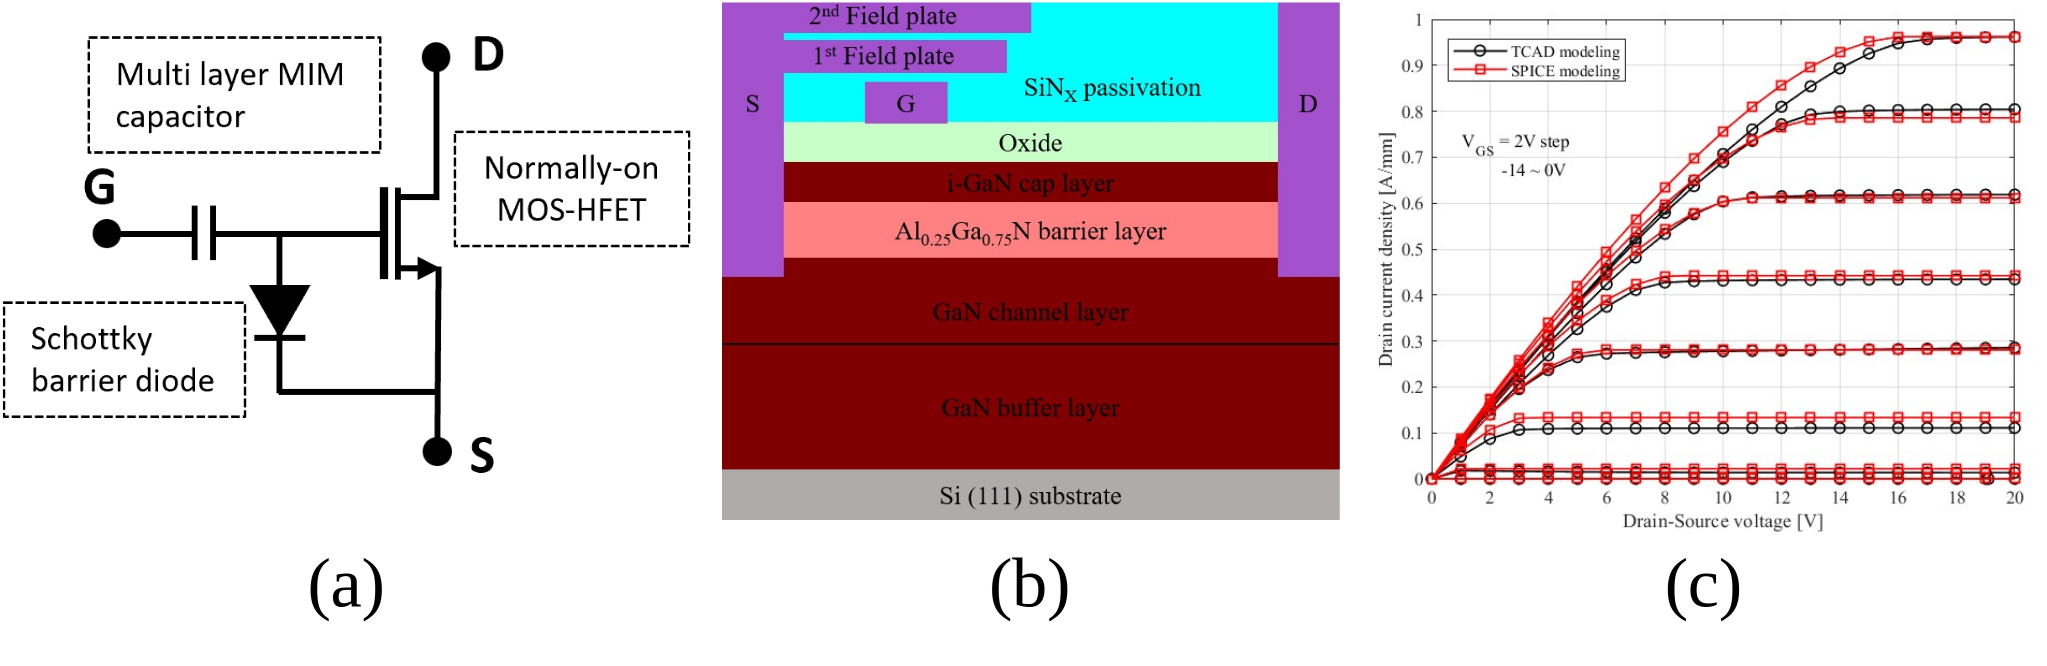
\includegraphics[width=6 in]{figures/figure5.pdf}
    \caption{
    (\textbf{a})
    Cross-section view of multi-layer trap and Maxwell simulation result on radial plane
    and
    (\textbf{b})
    Fabricated multi-layer ion trap
    }
    \label{fig:figure5}
\end{figure}

\begin{itemize}[leftmargin=2.0em]
    \item 
    \item 
    \item 
\end{itemize}

\begin{center}
    \subsection{Optimization of circuit}
\end{center}

\begin{figure}[h]
    \centering
    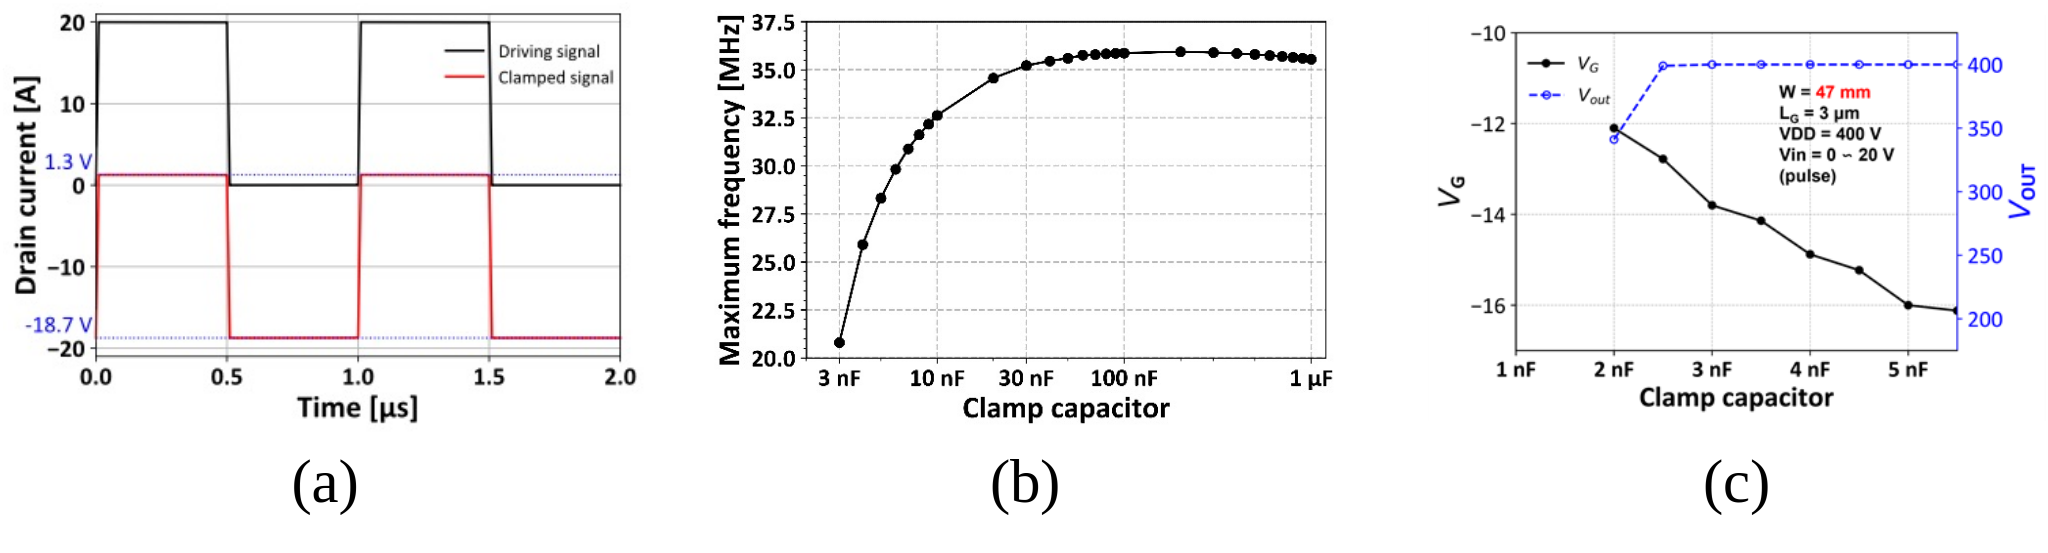
\includegraphics[width=6 in]{figures/figure6.pdf}
    \caption{
    (\textbf{a})
    Cross-section view of multi-layer trap and Maxwell simulation result on radial plane
    and
    (\textbf{b})
    Fabricated multi-layer ion trap
    }
    \label{fig:figure6}
\end{figure}

\begin{itemize}[leftmargin=2.0em]
    \item 
    \item 
    \item 
\end{itemize}

\begin{center}
    \subsection{DC-DC boost converter circuit}
\end{center}

\begin{figure}[h]
    \centering
    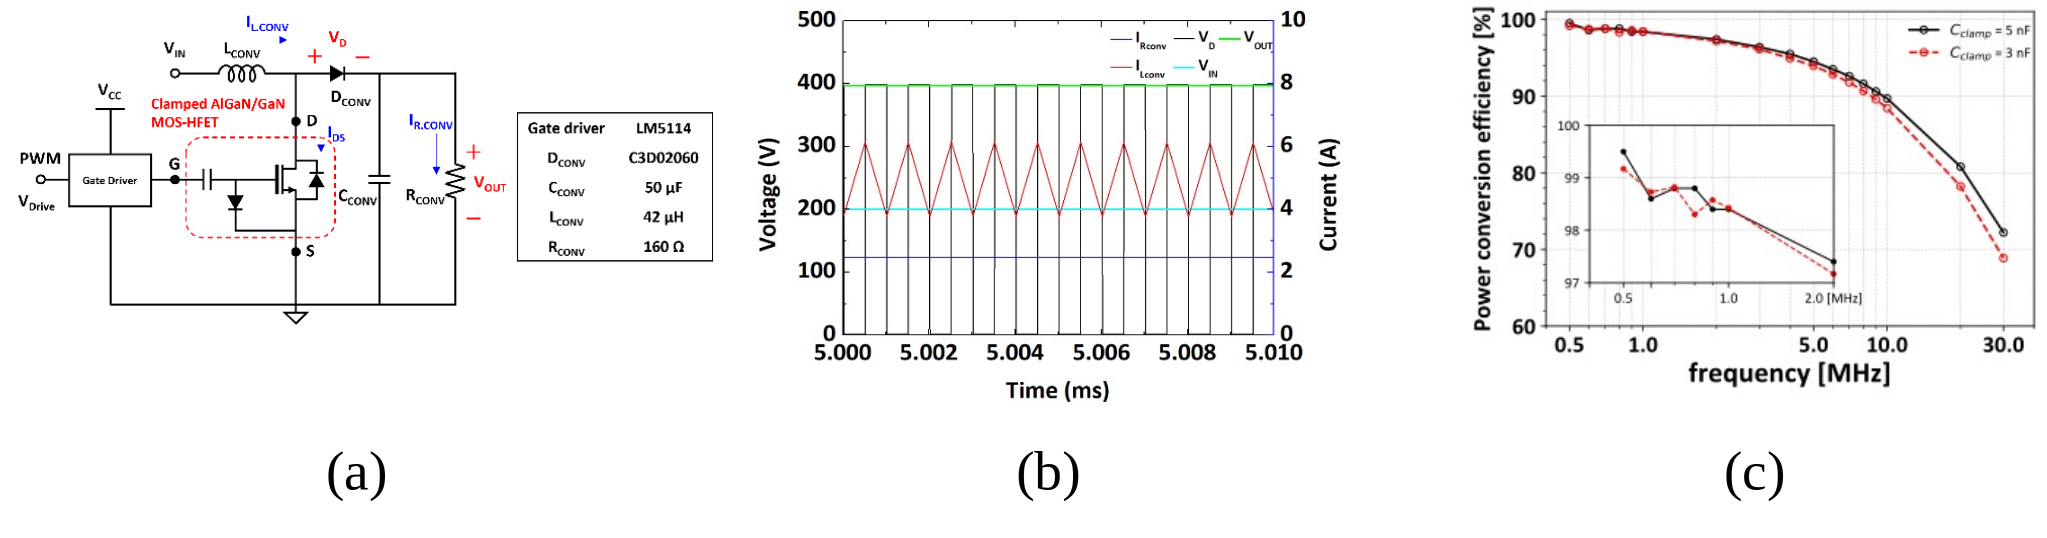
\includegraphics[width=6 in]{figures/figure7.pdf}
    \caption{
    (\textbf{a})
    Cross-section view of multi-layer trap and Maxwell simulation result on radial plane
    and
    (\textbf{b})
    Fabricated multi-layer ion trap
    }
    \label{fig:figure7}
\end{figure}

\begin{itemize}[leftmargin=2.0em]
    \item 
    \item 
    \item 
\end{itemize}

\end{document}